\chapter{绪论}\label{chapter01}
{\em 本章首先介绍研究的立项背景,分析保障数据隐私安全的重要性,并阐述研究意义。其次,综述分析差分隐私的国内外研究动态以及信息论、博弈论方法在差分隐私中的应用研究趋势。然后,围绕研究对象凝练出关键问题与目标。进一步,介绍本文的核心研究内容以及研究取得的主要成果。最后,给出具体章节组织安排。}
\section{研究背景与意义}
\subsection{研究背景}

数据安全是网络空间安全的重要组成部分,已成为互联网技术发展中亟需解决的关键问题。为保障网络信息安全,国家制定、公布、实施了《网络安全法》\cite{network2016}%\footnote{http://www.cac.gov.cn/2016-11/07/c\_1119867116.htm}
,其中涉及个人信息的使用、保护规范。在基于互联网的应用中(如社交网络、位置服务等),有关个人的数据不断地被收集、存储、利用,直接的分析、发布、共享这些个人数据将会导致个体隐私泄露问题。为建立健全个人信息安全保护管理制度,《互联网个人信息安全保护指南》\cite{individual2019}%\footnote{http://www.beian.gov.cn/portal/index}
明确了个人信息生命周期处理过程中的使用规范。该指南中对个人信息给出了明确的定义,个人信息生命周期阶段的操作做出明确的规范,目的是保障个人隐私信息安全。尽管如此,近年来个人隐私泄露事件依然频频发生,隐私泄露问题引发人们的困扰。下表 \ref{tab:privacyLeakageEvents_1.1}
调查列举了近三年主要发生的典型隐私泄露事件,由此可见,个人隐私保护的需求不断攀升。

\begin{table}[htbp]
\caption{近三年主要典型隐私泄露事件概览}
\label{tab:privacyLeakageEvents_1.1}
\centering
\fontsize{10pt}{\baselineskip}\selectfont
\begin{tabular}{p{0.12\textwidth}p{0.35\textwidth}p{0.35\textwidth}}%
	\toprule
	\textbf{发生时间}&\textbf{隐私泄露事件}&\textbf{泄露数据类型}\\
	\midrule
    2020年04月 & 青岛胶州中心医院就诊名单泄露 & 涉及6685人 的姓名、电话、身份证号码、居住地址、就诊类型等\\
	2020年03月 & 万豪连锁酒店数据泄露 & 包括姓名、生日、电话号码、旅行信息和忠诚计划信息\\
	2020年02月 & 美高梅酒店旅客信息泄露 & $10,683,188$名客人信息,包括家庭住址、电话号码、电子邮件和生日等\\
	2019年05月 & Clinical Pathology Laboratories 数据泄露事件 &泄露数据涉及姓名、地址、电话号码、出生日期、治疗信息等\\
	2019年02月 & Dubsmash 1.62 亿用户数据泄露 & 用户姓名、ID、用户名、密码等 \\
	2018年08月 & 华住集团旗下连锁酒店数据泄露 & 姓名、手机号、邮箱、身份证号等\\
	
\bottomrule
\end{tabular}
\end{table}

2020年10月,《中华人民共和国个人信息保护法(草案)》提请十三届全国人大常委会第二十二次会议审议,标志着个人隐私保护问题受到了政府和人民的高度重视,已成为一个普遍关注的热点问题。当前,解决个人隐私保护问题的途径主要有制定、完善法律法规和研究有效的隐私保护技术两个方面。在法律法规的规范引导下,隐私保护需要强有力的隐私保护技术支撑。为了深入理解具体的隐私保护技术方案,本文调查了不同应用场景下的隐私保护需求。社交网络\cite{wei2020asgldp,kasiviswanathan2013analyzing,jorgensen2016publishing}、地理位置\cite{oya2017back,zhang2019online,andres2013geo}、数据收集\cite{wang2016using,wang2019collecting,wang2017locally,wang2019local}、数据发布\cite{zhu2017differentially,qardaji2014priview}、数据挖掘\cite{agrawal2001on,agrawal2005privacy,wang2018locally}等应用中分别产生了用户社交关系、位置移动轨迹、敏感属性保密等隐私保护需求。针对这些场景中的隐私保护问题,学术研究提出了一系列的隐私保护技术方案。{\em 依据实现机理的不同,当前的隐私保护技术方案大致可以划分为三类:基于泛化和抑制手段的匿名类隐私保护、基于噪声扰动的差分隐私保护和基于密码方法的隐私保护}。首先,匿名类的隐私保护模型(如 ~$k$-anonymity \cite{sweeney2002k},$l$-diversity \cite{machanavajjhala2006l},$t$-closeness \cite{li2007t},($\alpha,k$)-匿名\cite{wong2006a},($k,e$)- 匿名\cite{zhang2007aggregate},($\epsilon,m$)-匿名\cite{li2008preservation}等)利用泛化和抑制
\cite{sweeney2002achieving}的手段实现基于准标识符的匿名等价类,降低了敏感数据泄露风险。然而,匿名类的隐私保护模型存在着难以抵御连接攻击、同质性攻击和相似性攻击的缺陷。大数据环境下,匿名类的隐私保护模型的局限性凸显。随后,为了解决统计数据库的隐私泄露问题,2006年~Cynthia~Dwork 提出了差分隐私(Differential Privacy,DP)\cite{dwork2006differential} 保护模型,旨在通过噪声扰动\cite{dwork2006calibrating}的方式实现相邻数据集上查询输出结果的$\epsilon$ 概率不可区分性。近年来,围绕隐私保护需求,研究者提出了诸多差分隐私保护方案,在隐私保护的数据发布 (Privacy-Preserving Data Publishing,PPDP)、隐私保护的数据分析(Privacy-Preserving Data Analysis,PPDA)、 隐私保护的数据挖掘(Privacy-Preserving Data Mining,PPDM)等场景中得到了广泛应用\cite{zhu2017differential}。总体上,差分隐私的研究工作主要是围绕噪声抽样分布和噪声扰动的方式展开,也就是研究差分隐私的噪声机制和最优化的隐私预算参数问题,其目的是为了平衡隐私保护与查询数据的精确度。此外,基于密码方法的隐私保护方案也得到了研究,如同态加密、密文搜索技术等 \cite{Lifenghua16}在隐私保护方案设计中得到了应用。但是,由于基于密码学的隐私保护方案存在计算复杂度较高的弱点,现阶段还无法满足实际应用中的时间和性能要求,因此尚未得到实际的广泛应用。表\ref{tab:comparisionPrivacyMechanisms_1.2}总结对比了三类隐私保护方法的特点。匿名类和差分隐私是现阶段主流的隐私保护模型。在现有的两类主流隐私保护技术中,敏感数据的隐私性与数据可用性是隐私保护方案设计的核心关注点,同时也是评价隐私保护机制的重要指标。

\begin{table}[htbp]

\caption{对比三类隐私保护方法}
\label{tab:comparisionPrivacyMechanisms_1.2}
\centering
\fontsize{10pt}{\baselineskip}\selectfont

\begin{tabular}{p{0.15\textwidth}p{0.20\textwidth}p{0.20\textwidth}p{0.35\textwidth}}
\toprule
	\textbf{方法类型}&\textbf{代表性技术}&\textbf{实现原理}&\textbf{方法特点}\\
	\midrule
  匿名类方法 & \makecell[l]{$k$-anonymity \\ $l$-diversity \\$t$-closeness\\ $\cdots$} &泛化、抑制&具有难以抵御连接攻击、同质性攻击和相似性攻击的缺陷 \\
随机扰动方法 & \makecell[l]{差分隐私\\ 本地化差分隐私\\ $\cdots$} &随机化扰动& 严格数学可证明的理论基础,提供最差情况下隐私保证\\
密码学方法 & \makecell[l]{同态加密\\ 可搜索加密 \\ $\cdots$} &加密、密文计算&计算复杂度较高,现阶段尚无法满足实际应用中的时间和性能要求 \\

  \bottomrule
\end{tabular}
\end{table}

近年来,差分隐私保护模型受到了学术界和产业界的热衷,其原因在于差分隐私提供了一种严格数学可证明的隐私保证,在最差的情况下(Worst-case)保障了特定个体的隐私信息被识别的概率不超过$\epsilon$因子。基于数据失真扰动的差分隐私中隐私度与可用性的权衡问题也一直是学术研究关注的焦点。针对该问题,设计有效的差分隐私方案是一种常见的解决方法。现有的研究工作提出了诸多的差分隐私方案,如几何机制\cite{ghosh2012universally}、Alvim等\cite{alvim2011differential}的最优随机化机制、互信息-隐私机制(MI-privacy)\cite{wang2016on,mir2012information}等。根据模型假设的不同可以划分为信息论方法和非信息论方法的研究。信息论的模型中对先验分布具有一定的假设,而差分隐私模型中没有考虑先验分布的影响\cite{sarwate2014a}。Dwork差分隐私模型\cite{dwork2006differential,dwork2006calibrating}提供分布独立的强隐私保障,其中的$\epsilon$-隐私度量仅依赖于条件概率分布。该模型无法捕捉隐私攻击者对数据具有的先验知识,为此,研究者提出了信息论的差分隐私模型。信息论的模型同时考虑了先验分布和差分隐私的条件分布对隐私泄露的影响,在此方面的研究已取得了一定的进展\cite{calmon2012privacy,sarwate2014a,cuff2016differential,wang2016on}。如Kalantari 等\cite{kalantari2018robust}考虑不同数据分布类型,研究提出了不同分布情况下对称机制和非对称机制的最优性。 由此可见,数据先验分布对差分隐私最佳机制设计的影响。
但是,目前的研究工作中还存在一些不足之处,尚需要深入的研究,主要表现为以下几个方面:首先,受隐私保护方案应用场景的影响,目前对于隐私的度量尚缺乏明确统一的定量化方法;其次,在面向多维属性或高维属性时,用户的隐私敏感度偏好、属性的相互关联以及相关程度等对隐私泄露、隐私机制的影响尚需要深入研究;进一步,在一些应用中,消息灵通的敌手以及含背景知识的敌手能力的表达以及对隐私泄露风险的影响需要考虑;此外,策略型的敌手能够适应的改变隐私推断策略,追求隐私最大化目标的策略行为也需要在隐私保护中考虑。这些存在的问题对当前差分隐私保护模型提出了研究的新课题。




\subsection{研究意义}
在个人信息保护备受重视的时代背景下,本文针对当前差分隐私模型在应用中面临的挑战,基于个人信息生命周期处理阶段,研究隐私数据发布阶段、数据收集阶段的差分隐私最优化机制问题具有重要的研究意义。

首先,本文针对具体的应用场景和敌手模型,基于信息论、优化与均衡理论开展隐私与效用度量、权衡隐私与效用的最优化模型与隐私机制设计、隐私机制评估与分析等方面的研究,为保护个人隐私信息安全提供一种技术支撑。基于信息量化的隐私度量和均衡优化角度的优化模型及算法为隐私泄露分析、隐私机制设计提供基础理论支撑。本文研究的均衡优化模型在理论上拓展了差分隐私研究的边界,丰富了差分隐私针对多维数据、关联数据、策略型敌手的隐私保护模型的研究。
其次,本文研究的模型求解算法在实践上可为差分隐私应用场景中隐私机制的设计与实现提供重要的参考。本文的研究恰合互联网信息服务中用户隐私保护的诉求,适应互联网技术发展阶段的个人隐私保护需求,对实现互联网数据隐私安全具有明确的现实意义。

\section{研究动态与趋势}
差分隐私(differential privacy,DP)是一种严格的隐私保护模型,为个体隐私信息提供了强隐私保障。标准形式的差分隐私\cite{dwork2006differential,dwork2006calibrating}定义相邻兄弟数据集的查询输出结果满足概率$\epsilon$-不可区分性($\epsilon$-indistinguishability),其中$\epsilon$ 是足够小的非负实数。差分隐私利用随机化的方式能够实现在保护个体隐私信息的同时保持数据的统计信息
\cite{dwork2006differential,dwork2006calibrating,dwork2008differential},现已逐渐成为数据隐私的标准。通常,{\em 差分隐私被划分为中心化差分隐私和本地化差分隐私两种架构模式}\cite{dwork2014algorithmic}。中心化模型(centered model)假设系统中存在一个可信的数据管理者能够访问原始数据,并利用隐私保护机制得到扰动数据。与之对应的,本地化差分隐私(local differential privacy,LDP)\cite{kasiviswanathan2011what,duchi2013local}是差分隐私(DP)的本地化应用,它是系统中无可信数据管理者的特殊情景。其主要应用于隐私保护的数据收集场景。在本地模型(local model)中,每个用户本地的执行LDP 隐私协议扰动其真实数据得到扰动数据(perturbed data),并将扰动数据报告给数据收集者。然后,数据聚合者收集、存储、分析这些用户上报的扰动数据。当前,差分隐私已成为隐私保护研究的标准,对其应用的研究涉及社交网络\cite{wei2020asgldp,kasiviswanathan2013analyzing}、推荐服务\cite{xiao2020deep}、移动众包计算\cite{sei2017differential}等领域,%隐私保护的数据类型从关系数据延申至图数据、键-值型数据、地理数据等不同数据类别。
图\ref{fig:chapter02-application-research}描绘了差分隐私的主要应用领域和具体场景中的核心研究问题。
本文中,围绕个人数据生命周期阶段,结合差分隐私的具体应用场景,{\em 从隐私保护的数据发布、隐私保护的数据收集、隐私保护的数据分析}角度介绍目前国内外学术研究的动态与趋势。%随后,本文分析了在差分隐私的应用研究中需要关注的关键问题。

\begin{figure}[htbp]
	\centering
	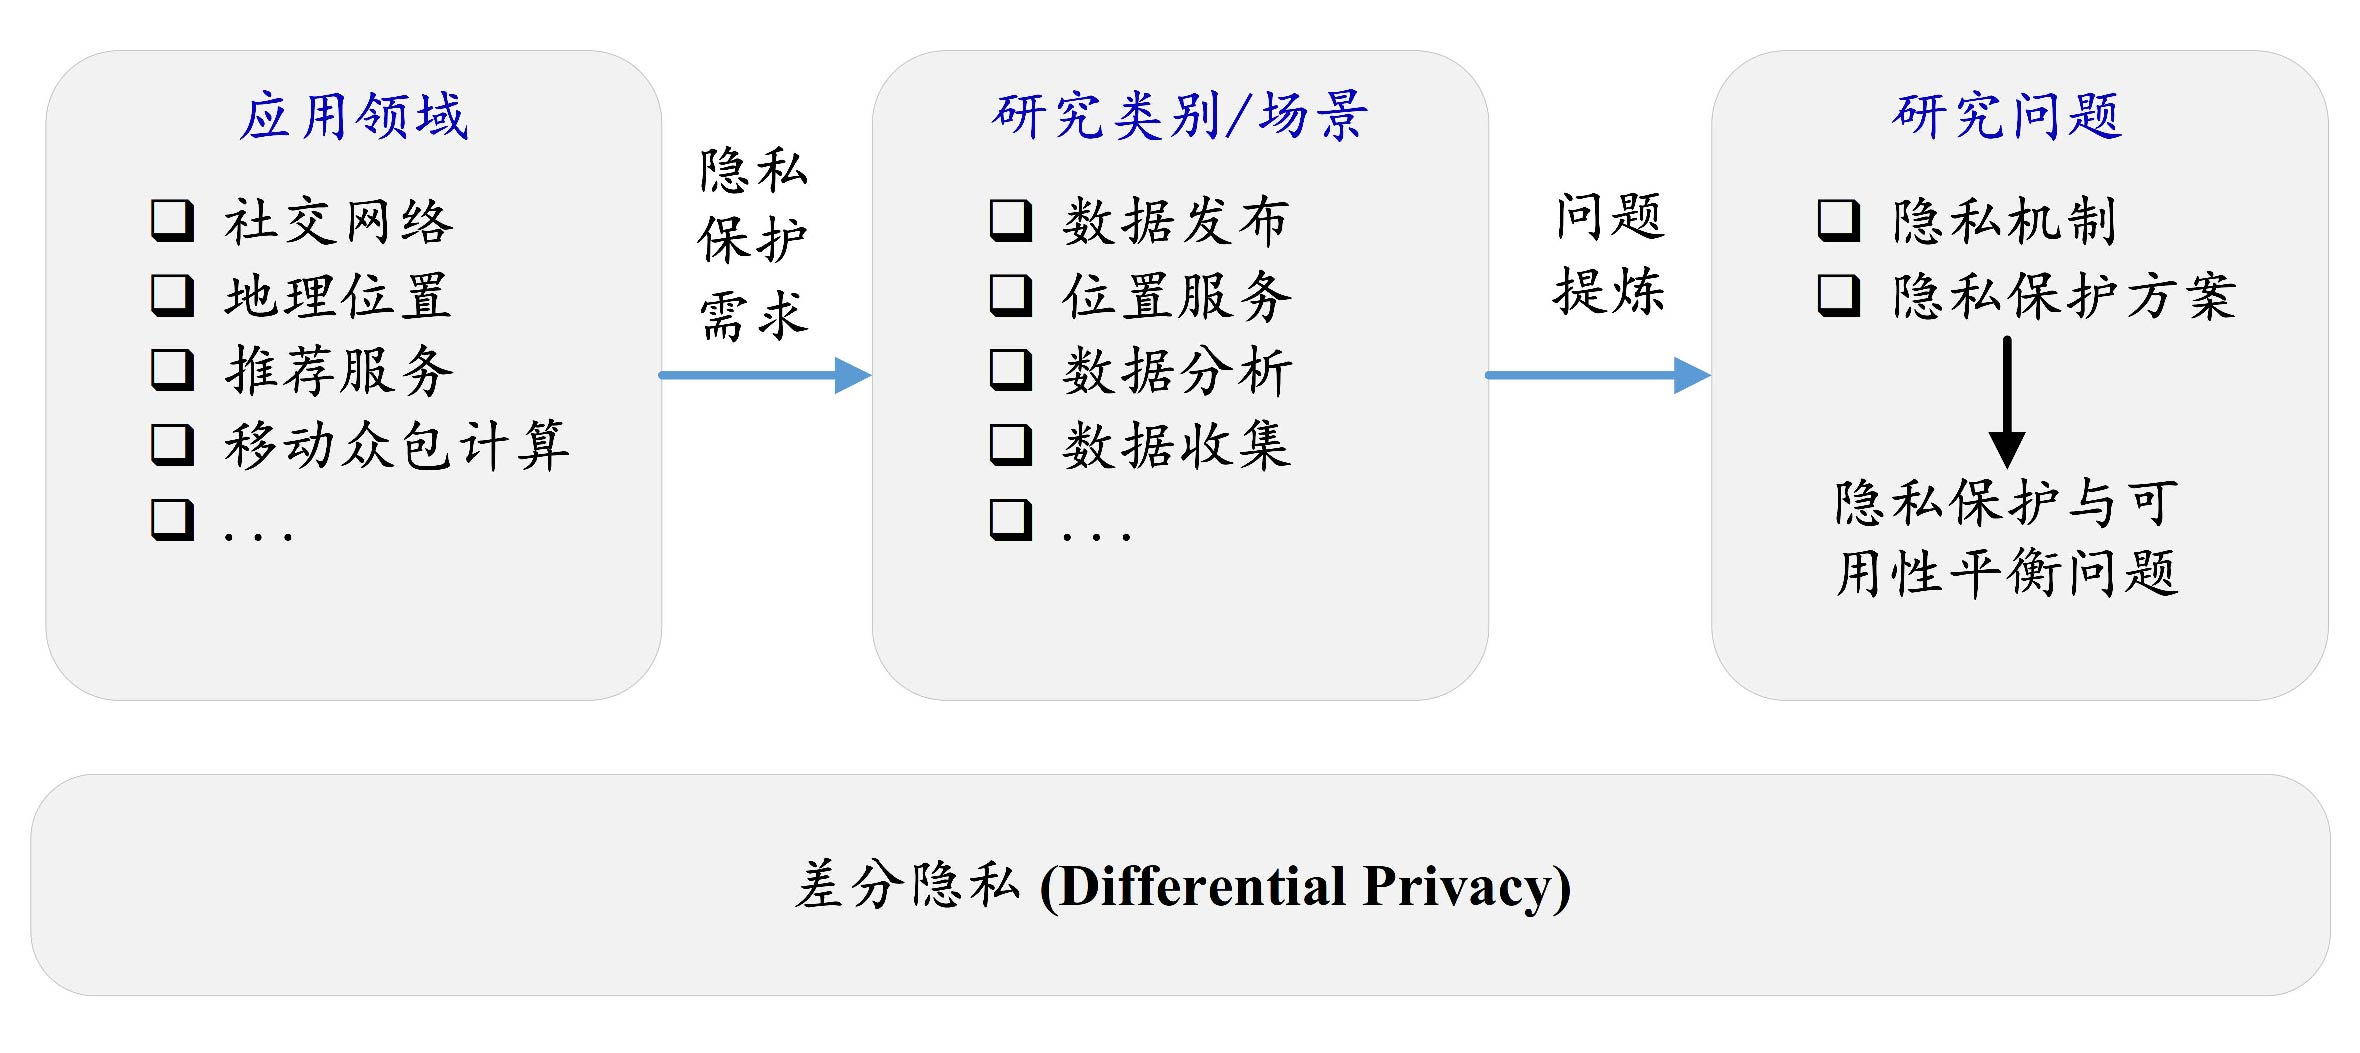
\includegraphics[width = 0.85\linewidth]{./figures/chapter02_3.jpg}
	\caption{差分隐私的应用研究}
	\label{fig:chapter02-application-research}
\end{figure}

接下来,综述近些年差分隐私应用研究中与本文研究相关的主要代表性成果,进一步分析差分隐私研究的发展趋势。

\subsection{研究动态}
差分隐私的基本思想是在隐私数据中引入随机性来阻止个人的信息被推断。显然地,随机化的程度越高,隐私保护效果越好,对应的数据可用性则降低。这就是隐私与效用原则\cite{sankar2013utility},也就是著名的隐私与效用权衡问题\cite{basciftci2016on,alvim2011differential}。该问题是隐私保护研究关注的核心问题,学术研究者围绕该问题做出了一系列有意义的研究工作。这些工作大致可以分为寻找更加有效的扰动机制\cite{ghosh2012universally,wang2016on,alvim2011differential}和研究有效的噪声注入方式\cite{geng2016the}两类。如文献\mycite{ghosh2012universally} 提出了几何机制(Truncated $\frac{1}{2}$-geometric mechanism)实现最优的差分隐私扰动。为了提高数据效用, 文献\mycite{xiao2011differential}提出在注入噪声之前,对数据进行小波变换(Wavelet Transforms),克服了Dwork方案中Laplace噪声扰动大的问题。文献\mycite{xu2017dppro}利用随机投影的方式研究了差分隐私高维数据发布的问题,解决了扰动误差大的问题。结合具体的应用场景,以下阐述差分隐私的学术研究动态。

首先,隐私保护的数据发布场景中,可信数据管理者发布数据以供进一步的数据分析\cite{aggarwal2008privacy},目标是发布数据的聚合信息而不泄露用户的个体隐私。差分隐私的数据发布包含有交互式发布和非交互式发布两种类型,其中,交互式数据发布包含有事务型数据发布、直方图数据发布、流数据发布、图数据发布;非交互式数据发布主要有批量查询发布、合成数据集发布\cite{zhu2017differentially}。隐私保护的数据发布场景中,发布数据的精确度与隐私泄露权衡是主要关注的核心问题。{\em 为了解决数据发布中存在的隐私泄露问题,差分隐私的机制是研究的核心关注点}。近年来,以Dwork的方法
\cite{dwork2006calibrating}为基础,针对不同的发布数据类型,研究者提出了诸多的差分隐私数据发布模型及算法。
表\ref{tab:survey_dp_publishing}列出了差分隐私数据发布的主要部分研究工作。

\begin{table}[htbp]
\caption{差分隐私的数据发布方法}
\label{tab:survey_dp_publishing}
\centering
\fontsize{10pt}{\baselineskip}\selectfont
\begin{tabular}{p{0.10\textwidth}p{0.05\textwidth}p{0.30\textwidth}p{0.30\textwidth}}
\toprule
	\textbf{工作模式}& &\textbf{数据发布类型}&\textbf{主要研究}\\
	\midrule
   交互式数据发布& &\makecell[l]{事务型数据发布 \\ 直方图数据发布 \\ 流数据发布\\ 图数据发布} &\makecell[l]{
IDC\cite{gupta2012iterative}\\Laplace\cite{dwork2006calibrating},Partitioning\cite{chen2011publishing}\\ Pan-Privacy\cite{dwork2010differential},P-Sums\cite{chan2011private}\\ Edge DP\cite{zhang2015private}, Node DP\cite{kasiviswanathan2013analyzing}} \\
   \midrule
非交互式数据发布& &\makecell[l]{批量查询发布\\ 合成数据集发布} & \makecell[l]{Batch Query\cite{yuan2012low}\\ Sanitization\cite{dwork2009on}}\\

  \bottomrule
\end{tabular}
\end{table}

其次,本地化差分隐私的应用研究\cite{yeqingqing2018}已逐渐成为差分隐私的另一个重要研究方向,在隐私保护的数据收集、数据发布场景中都得到了不同程度的应用。围绕本地化差分隐私的应用,主要是研究如何设计可获得的隐私机制实现预期的目标。本地隐私模型中,随机化响应(Randomized Response,RR)\cite{warner1965randomized}技术是一种获得LDP的有效方式,现已发展成为本地化差分隐私机制设计的基本构建模块,在本地差分隐私中的应用取得了显著的效果。近年来,很多著名的LDP隐私机制(如$k$-RR \cite{kairouz2016extremal},$O$-RR\cite{kairouz2016discrete},RAPPOR \cite{erlingsson2014rappor,fanti2016building},MeanEst\cite{duchi2013localprivacy}等)已经被研究者提出。周异辉等\cite{zhouyihui2019}针对隐私-效用均衡问题,从优化理论的角度给出了效用优化模型,并分析了随机响应机制的最优性条件和相应的效用最优机制。此外,对于其它数据结构的本地化差分隐私也得到了研究,如set-value的本地化差分隐私
\cite{wang2018privset,qin2016heavy}、key-value类型数据的本地化差分隐私\cite{ye2019privkv}以及图数据结构的本地化差分隐私\cite{wei2020asgldp}。本地化差分隐私的应用涉及到社交网络\cite{qin2017generating}、移动众包计算\cite{sei2017differential}、数据合成发布\cite{ren2018textsf,yang2017copula}等场景,也因此日渐受到关注。本地化模型中,攻击模型通常被假设为半诚实(Semi-honest)的敌手模型,也就是说,数据聚合者诚实的执行隐私协议但是试图从报告的扰动数据中推断用户个体的隐私信息\cite{sei2017differential}。在本地化模型中,隐私与效用的权衡问题仍然是学术研究关注的重点。

最后,隐私保护的数据分析是在保持数据分析的精确度的同时保护个体的隐私信息\cite{wang2016on}。近年来,基于学习理论的方法在差分隐私中得到了具体的应用,包括数据分析与机器学习的方法在差分隐私中的应用\cite{kasiviswanathan2011what,ye2017optimal,sarwate2013signal}(如概率分布估计\cite{Murakami2018Toward},数据训练\cite{xu2019ganobfuscator})。2018年,Ren 等\cite{ren2018textsf} 使用~(Expectation Maximization,EM)~和~Lasso~的方法进行分布估计,用于得到联合概率分布,支撑发布数据集合成。2019年,Wang等\cite{wang2019collecting}基于机器学习的线性回归(Linear Regression)、逻辑回归(Logistic Regression)、支持向量机(Support Vector Machines,SVM)分类算法分析了所提出分段机制(Piecewise Mechanism,PM)和混合机制(Hybrid Mechanism,HM)的性能。由此可知,隐私保护的数据分析主要是学习数据的统计特征,体现出扰动数据的质量。

鉴于上述分析可知,差分隐私在隐私保护中占据着重要的地位,它已经涉及到了具有隐私保护需求的各种信息系统应用。现阶段,差分隐私在面向低维数据和独立同分布数据情景的研究相对比较成熟。针对低维的数值型数据和类别型数据,目前已有诸多的隐私保护方案(如Duchi等人\cite{duchi2018minimax}提出的数值型方案,Wang等人\cite{wang2017locally}提出的类别型Optimized Unary Encoding,OUE方案)。但是,随着应用系统的需求升级,面向多维数据且存在数据关联的情景时,直接地拓展当前的方案到多维情景,则会面临性能和效用降低的挑战。此外,多维属性的用户隐私敏感偏好表达也是亟待解决的问题。针对这些问题,研究者积极的探索新的解决方案,以下给出研究进展及现状的介绍。



(1) {\em 面向多维数据的差分隐私}

随着用户数据维度的增加,多维或高维数据具有笛卡尔乘积空间大、数据稀疏性的特点,给差分隐私数据处理带来新的挑战。具体地说,差分隐私对于多维数据或高维数据的处理主要面临着隐私脆弱性、计算复杂度高等问题。为了解决这些问题,数据降维是一种通常采用的处理方法。将有关个体的数据元组,拆分为多个属性分量,然后独立的应用差分隐私机制,该处理思想以差分隐私的并行组合原理\cite{dwork2014algorithmic}为基础,其基本的处理流程如图\ref{fig:chapter02-multidimension-data}描述。

\begin{figure}[htbp]
	\centering
	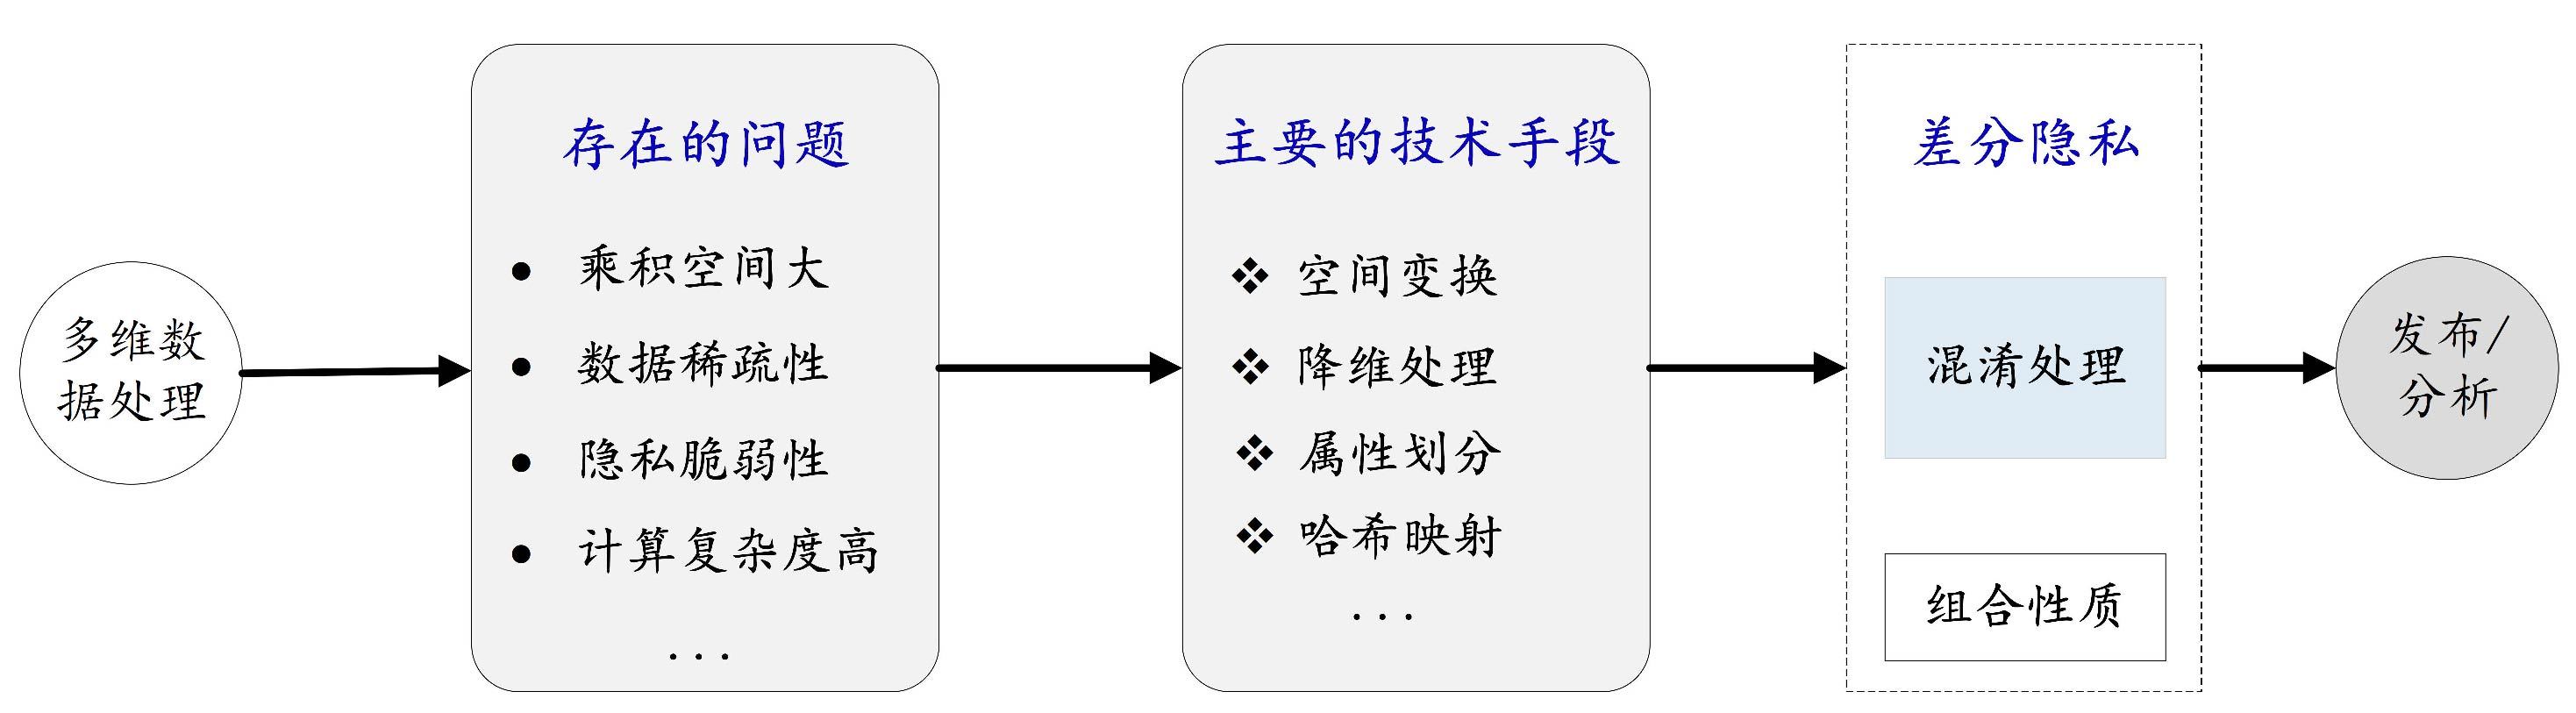
\includegraphics[width = 0.85\linewidth]{./figures/chapter02_4.jpg}
	\caption{差分隐私多维数据处理流程}
	\label{fig:chapter02-multidimension-data}
\end{figure}

针对差分隐私的多维数据处理,研究者做了一些有意义的探索,提出了差分隐私的多维数据处理方案。2017年,Xu等\cite{xu2017dppro}针对多维数据发布中存在的扰动误差增加和计算复杂性问题,通过随机投影的方法提出了高维数据发布的DPPro方案。此外的本地化差分隐私模型中,Wang等\cite{wang2019collecting}针对多维数据的收集和分析场景,推广并改进了Duchi等人\cite{duchi2018minimax}的方案,提出了分段机制(PM)和混合机制(HM),其思想是将属性分为数值型和类别型数据,然后依赖于单一数值型扰动方案和存在的任意类别型扰动方案(如OUE\cite{wang2017locally}),实现多维混合数值型和类别型数据的处理。Ren等\cite{ren2018textsf}将基于Bloom Filter和RR实现的RAPPOR机制拓展应用到高维数据情景,利用属性值拆分、扰动合并和差分隐私的组合定理\cite{kairouz2017the},考虑了差分隐私高维数据发布的问题,提出了LoPub。其基本思想是将元组进行属性拆分,然后利用Hash函数和Bloom Filter映射属性值到比特串,并逐比特的进行随机扰动,产生扰动的元组。该方法首先将原始数据哈希得到``0''和``1''的比特串,然后随机响应实现随机的扰动。Yang等\cite{yang2017copula}基于随机响应技术本地转化用户数据到比特串,实现多维数据合成和发布的机制。事实证明这是一种相对有效的处理方法,且被广泛的应用在隐私保护的多维数据情景。该思想在基于地理位置的隐私保护系统中也有相应的应用。如混淆扰动一个元组时,独立的应用存在的隐私保护机制到元组的每一个位置点,然后得到整个响应的混淆元组\cite{andres2013geo}。近年来,面向多维数据的差分隐私研究逐渐成为一个重要的研究点,但是,目前针对混合数值型和类别型多维数据处理的差分隐私最优化机制的研究还相对较少。面向多维数据处理的差分隐私机制设计仍然是一个重要的研究方向,尚需要进一步的研究。


(2) {\em 面向数据关联的差分隐私}

现有的差分隐私处理方法大多假设数据抽样独立,然而实际应用中,多维数据通常不是独立存在,而是存在着相互关联的情况。事实上,这些关联可以分为数据的记录关联、属性关联或隐私攻击者的关联辅助背景知识关联等情况。文献\mycite{kifer2011no}揭示了相关数据上的隐私机制将比期望的泄露更多的信息。为此,近些年数据关联的差分隐私机制设计问题受到研究者关注。

{\em 例如,数据集中属性年龄、职业可能和婚姻状态存在属性关联,这种关联使得敌手能够以较高的置信推断用户的隐私信息,从而增加隐私泄露风险。针对数据关联隐私泄露问题,文献}\mycite{zhu2015correlated}{\em 揭示由属性导致的元组相关,增加了流感疾病隐私泄露风险;文献}\mycite{li2019impact}{\em 分析了敌手背景知识对隐私泄露的影响。}针对数据关联的隐私泄露影响,研究者开展了相关的研究工作。
2014年,Zhang 等\cite{zhang2014privbayes}利用贝叶斯网络考虑了数据集属性关联的情景,借助互信息分析属性之间的相关度\cite{reshef2011detecting,liangjy2016},提出利用贝叶斯网络实现差分隐私的高维数据发布。2015年,Zhu等\cite{zhu2015correlated}针对非独立同分布的数据集记录关联,改进了差分隐私的敏感度计算方法,减少了噪声注入提升了数据效用。Yang等\cite{yang2015bayesian}研究了数据相关对隐私的影响,敌手先验知识对隐私的影响和数据相关时的扰动算法设计,提出了贝叶斯差分隐私。2017年,Song等\cite{song2017pufferfish}提出Pufferfish privacy保护关联数据的隐私。2019 年,Li 等\cite{li2019impact} 基于皮尔逊的相关度分析方法,从强关联、弱关联、正相关和负相关的角度,考虑了隐私攻击者的背景知识和数据关联对差分隐私数据发布的影响。鉴于上述分析,由数据的记录关联、属性关联或隐私攻击者的关联辅助背景知识,导致的隐私泄露问题,或是存在数据关联的高维数据发布问题仍然是学术研究关注的焦点。数据相关的隐私度量分析成为隐私机制设计首要解决的问题。

(3) {\em 面向用户偏好的差分隐私}

差分隐私模型扩展应用于多维数据时,差分隐私的隐私特性($\epsilon$-度量)由其组合性质保障。通常情况下,差分隐私把多维属性看作等价敏感,提供相同等级的隐私保护。例如,用户个体的隐私数据包含$d$个属性维度,差分隐私机制的隐私预算设置$\epsilon/k$,然后依据序列组合性质,隐私保护总体满足$\epsilon$- 差分隐私。但是,多维的属性之间可能存在不同的隐私敏感度,也就是用户的隐私敏感偏好。为了更好的阐述这个问题,首先给出以下问题引例。

{\em 假设个体数据元组由年龄、性别、教育程度、婚姻状态组成,这些数据项都是有关个体的隐私信息。但是,在这些数据项中,用户对其数据具有不同的隐私感受。通常情况下,一个人的性别可能不被认为是隐私数据或者具有较低的隐私敏感性。然而,一个人的婚姻状态(如离婚)是想保持私密性的敏感数据,其隐私私密性高于其它属性。}为了能够解决诸如此类的问题,这就要求差分隐私能够提供不同敏感等级的隐私保护对于有区分的属性,满足所提出的隐私保护需求。

针对上述问题,研究者依据属性敏感度等级,提出了有区别隐私数据的个性化差分隐私保护方案\cite{chen2016private}。2015年,Jorgensen等\cite{jorgensen2015conservative}考虑个人数据的不同隐私保护需求,提出了个性化差分隐私(Personalized Differential Privacy,PDP)的概念。2019 年,Wang 等\cite{wang2019personalized}利用泛化的$d_{\mathcal{X}}$-privacy\cite{chatzikokolakis2013broadening}研究了个性化隐私保护。Murakami 等\cite{murakami2019utility} 提出了效用最优的本地化差分隐私方案(Utility-optimized LDP,ULDP)用于隐私保护的数据收集与分析。通过划分个体数据为敏感数据和非敏感数据两部分,推广Mangat\cite{mangat1994an}随机响应到多元字母表情景,提出了ULDP方案,对于敏感数据提供和LDP 等价的隐私保障。2020年,Gu 等\cite{gu2020providing}通过考虑不同输入数据具有不同的隐私敏感度,提出了一种输入区分(Input-discriminiative)的隐私保护机制(Input-discriminiative LDP,ID-LDP)。由此可见,考虑用户隐私偏好,设计差分隐私机制,实现为不同敏感度的用户数据提供有区分的隐私保护成为一种新的研究方向。


\subsection{研究趋势}
Shannon\cite{shannon1948a}为解决信息度量问题提出信息熵的概念之后,信息熵在通信、密码学等领域发挥了重要的作用。近年来,基于信息度量的量化信息流思想(Quantitative Information Flow,QIF)\cite{smith2009on}逐渐在隐私保护中得到应用。此外,博弈均衡理论作为一种有效的分析工具在隐私保护中也得到了应用。针对差分隐私应用中存在的隐私与效用的平衡问题,基于信息论、博弈论以及交叉学科的方法开展研究逐渐成为一个重要的研究方向。以下从两个方面综述密切相关且具有代表性的研究成果。

(1) {\em 差分隐私的信息论方法}\label{subsec:information_dp}

隐私保护模型的本质是数据混淆、扰动机制,它可以表达为一种概率性的函数映射,与信息论的方法密切相关\cite{Duchi2019information}。由此,在隐私保护研究中,信息熵发展成为一种有效的隐私度量方法\cite{issa2016an,Chatzikokolakis2008Anonymity}。以信息熵为基础定义的R\'{e}nyi熵\cite{renyi1961on,erven2014renyi,mironov2017renyi}、条件熵、联合熵、互信息量等在隐私保护研究中得到了应用\cite{wang2019consistent,mcgregor2010the,du2015Fundamental,lopuhaa-zwakenberg2019information}。{\em 首先,隐私度量方面},Mir 等\cite{mir2012information}利用信息熵、条件熵、互信息量研究了隐私信息的度量问题,奠定了差分隐私的信息论方法研究基础。Barthe 等\cite{barthe2011information} 利用信息熵研究了差分隐私的隐私边界问题。Issa等\cite{issa2016an,2016Maximal}提出Maximal leakage方法测量隐私泄露,随后,Liao等\cite{liao2019tunable}对其扩展提出$\alpha$-leakage。{\em 其次,信息论的方法对于差分隐私的机制研究}也有一定的应用\cite{diaz2020on,kairouz2016extremal,wang2016on}。2011年,Alvim 等\cite{alvim2011differential,alvim2011on,alvim2015on}几乎是最早提出基于量化信息流(QIF) 的思想,将信息熵应用到差分隐私中量化隐私信息的不确定度,抽象差分隐私噪声机制为信息论噪声信道,并从信息论的角度考虑了平衡隐私度与数据效用的方法,同时提出信息论对称信道机制能够达到理论上的最优性。{\em 随后,信息论方法研究的差分隐私与标准差分隐私之间的关系}得到研究者关注\cite{mcgregor2010the}。Cuff 等\cite{cuff2016differential}基于互信息的概念给出了与标准差分隐私等价的信息论差分隐私定义。文献\mycite{calmon2012privacy,makhdoumi2013privacy}研究建立了互信息约束与差分隐私的关系。进一步,Wang 等\cite{wang2016on}提出可辨识识别(Identifiability)的概念、并研究了与差分隐私(Differential Privacy) 和互信息隐私(Mutual Information Privacy) 三个不同隐私概念之间的基本联系。{\em 更重要地是,信息论中著名的信源编码定理、限失真编码定理(保真度准则)}\cite{cover2006elements}{\em 在隐私保护中均得到了相应地研究}\cite{rebollo-monedero2010from,du2015Fundamental}。如Sankar等\cite{sankar2013utility}针对统计数据库隐私泄露问题,构建了统计数据库的概率模型,从最佳信源编码、译码方案的角度考虑了信息论方法在数据库中平衡隐私与效用的应用。在允许部分失真的情况下,最小信息传输率的率失真理论在差分隐私\cite{mir2012information,wang2016on}最优机制研究中也受到了关注。

随机响应技术是实现本地化差分隐私的有效方法,信息论方法对于随机响应的研究也得到了广泛的应用。事实上,本地化差分隐私的随机响应实现是根据特定的概率密度函数(Probability Density Function,PDF)随机响应。在此方面的研究关键在于设计满足差分隐私的概率密度函数。{\em 近年来,信息论方法的研究已从二元随机响应发展到多元随机响应,逐步向复杂数据类型拓展延伸}。具体的研究工作从信息论的本地化差分隐私度量
\cite{lopuhaa-zwakenberg2019information},向最优机制设计发展。Sarwate 等\cite{sarwate2014a}抽象二元离散随机响应机制为Shannon 信息论\cite{shannon1948a}离散噪声信道,基于率失真理论\cite{cover2006elements} 对本地化差分隐私的二元随机响应机制进行了研究,指出对称信道机制能达到最优性。但是,二元随机响应仅能处理`` 是''和``否''的问题,其应用具有局限性。随后,研究者对其进行了拓展研究,发展了多元随机响应(Multivariate Randomized Response,MRR) 技术。Kairouz等\cite{kairouz2016extremal} 基于互信息提出了$k$-RR机制,并在此后被进一步研究,发展了一系列先进的差分隐私机制。Kalantari 等\cite{kalantari2018robust}考虑不同先验概率分布情况,研究了汉明失真下平衡隐私度与数据效用的最佳差分隐私信道机制问题,指出对称信道机制和非对称信道机制的最优性对不同分布的最优性。Xiong 等\cite{xiong2016randomized}在隐私保护的数据收集场景,利用信息论的方法,将差分隐私的数据扰动机制抽象为离散无记忆的噪声信道机制,从限失真约束条件定义差分隐私信道集合,研究了本地化差分隐私的机制问题。

{\em 基于这些相关的研究工作,可以看出信息论的方法应用于差分隐私研究,主要是解决两个方面的问题}:(1) {\em 隐私信息的度量问题};(2) {\em 差分隐私的机制设计问题}。首先,前者的研究主要是从熵的内涵角度理解隐私泄露问题,该研究可用于评估隐私泄露风险(例如,定量分析隐私泄露的界),同时也是信息论方法对差分隐私机制研究的基础;其次,为了解决隐私与效用的平衡问题,后者的研究主要关注于最优的差分隐私实现机制。对于该问题的解决,信息论方法是从噪声信道角度寻找满足给定约束条件的最优条件概率分布。由此,基于优化理论建模\cite{iyengar2019towards}、求解该问题是一种理想的选择。如极大极小定理、Karush-Kuhn-Tucker (KKT)条件等\cite{boyd2004convex}得到了具体的应用。结合凸性或拟凸性形式化隐私与效用平衡问题为拟凸优化问题\cite{xiong2016randomized}、隐私失真最优化问题\cite{wang2016on}(信息论领域的率失真问题)
是较好的解决方法。但是,现阶段信息论方法总是假设数据抽样独立,对多维数据情景、多维属性存在关联、混合数值型和类别型的最优差分隐私机制问题尚未充分研究。

(2) {\em 差分隐私的博弈论方法}

隐私与效用的平衡问题(Privacy-utility Tradeoff)是隐私保护数据收集、隐私保护数据发布等应用场景中广泛关注的矛盾冲突问题。直观地,隐私保护效果越好,则噪声扰动导致的数据质量损失越大,从而数据效用降低。反之,数据效用越高,则隐私保护强度减弱,由此引发的隐私泄露量较大,这被称为隐私与效用原则\cite{sankar2013utility}。在隐私保护的模型与算法研究中,如何平衡隐私与效用是一个研究的关键问题。针对此,上述优化理论的方法是一种行之有效的解决方案。除此之外,基于最优性发展起来的博弈论\cite{Neumann1944The}也为隐私保护提供了有效的分析手段。博弈分析方法从理性的角度分析存在矛盾冲突情景下的参与者最优策略选择问题。近年来,在差分隐私研究中得到了一定程度的应用,其基本思想是分析隐私保护系统中参与者的理性行为,以均衡的思想解决隐私保护与数据效用平衡问题。

2013年,Hsu等\cite{hsu2013differential} 在差分隐私框架下针对隐私查询发布问题,建立了数据拥有者和数据查询者之间的两方零和博弈模型,提出一种新的隐私机制。2017年,Wu等\cite{Wu2017Game}构建了一个多方的有限策略型博弈,利用纯策略纳什均衡的存在性条件\cite{Glicksberg1952A}研究了差分隐私关联数据集发布的隐私预算参数选取问题。2019年,Qu等\cite{cui2019improving}针对隐私与数据效用之间的权衡问题,提出了一种基于社会距离的个性化差分隐私方法,在用户和敌手之间建立了静态贝叶斯博弈,从贝叶斯纳什均衡的角度权衡隐私与效用。此外,非合作的微分博弈\cite{gao2019a}和斯坦伯格博弈(Stackelberg)\cite{fioretto2020differential,shokri2015privacy} 也都在差分隐私中得到了研究。值得强调的是,Alvim 等\cite{alvim2017information,alvim2018leakage}基于量化信息流的思想,采用信息论方法度量隐私泄露,构建了隐私保护攻击与防御的两方零和博弈模型,进一步,基于极大极小理论\cite{du1995minimax}分析了隐私防护者与隐私攻击者的最佳策略选择。该研究工作将信息论的方法融入到博弈模型中,标志着一种新的研究趋势。但是,该研究工作没有针对具体的差分隐私保护模型展开研究,因此,在该方面仍然存在较大的研究提升空间。博弈模型用于差分隐私的研究,关键问题在于分析具体应用场景中隐私保护参与者和策略集,定义合理的收益函数,解决均衡的问题。

\section{关键问题与目标}



相关研究工作表明信息论度量方法、有损压缩\cite{xiong2016randomized,sarwate2014a}方法用于量化隐私泄露,研究隐私机制具有较好的优势。但是,在面向多维数据处理时,多维属性及相关性给差分隐私机制带来新的挑战。目前的研究尚未充分解决多维数据关联的隐私度量,缺乏敌手关联知识辅助推断用户隐私的定量化研究和隐私攻击者(敌手)拥有关联背景知识情景下的最优化隐私机制研究。此外,当前差分隐私保护系统中主要考虑敌手观察扰动数据后的被动攻击行为\cite{alvim2017information},较少考虑敌手的隐私攻击策略对系统的影响。基于此,本文聚焦在差分隐私应用中面临的核心热点问题。{\em 受已有工作的启发,本文利用信息论、博弈均衡理论、优化理论的方法,从基础的隐私度量、优化模型、算法设计等方面研究差分隐私最优化隐私机制问题,力图为差分隐私应用中权衡隐私与数据效用提供一种基于均衡、优化的理论支撑。}为了实现本文目标,提炼出以下4个关键问题:


(1) {\em 隐私与效用的度量}

围绕隐私保护中隐私与效用之间的权衡问题,对数据隐私与效用的合理度量是研究隐私保护机制的基础,但是,由于应用场景的复杂性,隐私信息在不同应用中难以被准确刻画,存在隐私度量缺乏定量化定义\cite{Lifenghua16}的问题。事实上,隐私泄露分析与敌手攻击模型密切相关,不同的系统模型和敌手模型下,隐私与效用的度量应该表达出敌手的隐私偏好和隐私推断能力。重要的是,隐私与效用的度量是研究隐私与效用权衡问题的一项基础且关键的工作,同时也是建立后续模型的基础。因此,隐私与效用的度量成为一个首要解决的关键问题。

(2) {\em 权衡隐私与效用的优化模型}

根据隐私与效用原则\cite{sankar2013utility},隐私保护中的隐私与数据效用之间存在相互依存且矛盾对立的关系,同时,它们也是隐私保护机制的两个重要评价指标。针对此,采用优化理论的方法寻找一个最优的权衡折中是理想的解决方法。但其关键在于如何将它们形式化为一个约束条件下目标函数最小化形式的可求解问题。如差分隐私数据发布场景中,约束质量损失函数在一定的阈值,最小化隐私泄露的优化模型是一种解决方案。由此可见,在不同的敌手模型下,形式化隐私与效用的权衡问题为具体的优化模型是隐私保护机制设计的关键。针对不同的敌手模型和差分隐私应用场景,差分隐私的机制设计仍需要更进一步的研究。

(3) {\em 隐私保护机制的设计}

设计合理的隐私机制是隐私保护的一个核心研究内容。目前的差分隐私随机概率映射机制,大多是具有某些特殊性质的条件概率分布集合,如对称机制\cite{kalantari2018robust}、$k$-RR\cite{kairouz2016extremal}机制等。如果在差分隐私应用中考虑敌手可能拥有的先验分布知识,则最优化的隐私机制需要考虑数据先验分布的影响。隐私机制设计
依赖于先验分布而独立于隐私数据。针对诸如此类的需求,通过隐私分析建立优化模型,求解计算最优隐私保护机制的概率密度函数是一种解决方案。此外,对于优化问题的计算方法,计算开销,以及推广到多维或高维数据时的隐私机制设计都需要进一步的研究,这是完成隐私保护方案设计的关键。


(4) {\em 隐私保护机制的评价方法}

隐私保护机制的评价是衡量隐私保护效果的重要方法,涉及到隐私度与数据质量两个方面。通常情况下,隐私度与数据质量(数据效用)是评价隐私保护机制的两个主要指标。在差分隐私中,不可分辨水平$\epsilon$和数据质量损失(如$l$-范数距离、均值平方误差、欧几里得距离、失真函数等)是主要的隐私和数据效用的评价指标。但是,不可分辨水平的$\epsilon$隐私度量仅依赖于差分隐私条件概率的比值。由此,$\epsilon$隐私度量面对等价的差分隐私机制时,则存在无法评价的问题。另外,在多维属性、数据关联的差分隐私处理环境中,属性的相关度测量以及相关度损失需要进行量化,它们也是评价差分隐私机制的重要指标。鉴于此,对于隐私保护机制的评价尚需要进一步的延伸拓展,需要结合具体的隐私保护系统模型评价隐私保护机制的性能。

\section{研究内容与成果}
%{\em 基于上述个人隐私保护背景以及当前差分隐私面临的问题,本节介绍本文的具体研究内容和相应的研究目标。}
%\subsection{研究内容}
围绕差分隐私应用场景中隐私与效用权衡的核心问题,本文研究差分隐私的最优化机制需要解决上述$4$个关键问题。为此,本文基于信息论方法、最优化理论以及博弈均衡理论研究提出了差分隐私的均衡优化模型及相应算法,实现隐私保护与数据效用的权衡折中。概括地说,本文的研究内容主要有:(1) {\em 差分隐私通信模型及其度量方法};(2) {\em 差分隐私均衡优化模型};(3) {\em 差分隐私均衡优化模型的算法}。三个研究内容相辅相成,具有较明确的内在逻辑性,下图\ref{fig:chapter1-research-relation}展现了本文的核心研究内容及其内在支撑关系。其中,研究内容(1) 为基础,支撑理论模型与算法的研究,研究内容(2)和(3)相互依赖并支撑计算最优隐私机制的概率分布,三者形成本文的核心研究内容,共同支撑外围差分隐私的应用。
\begin{figure}[htbp]
	\centering
	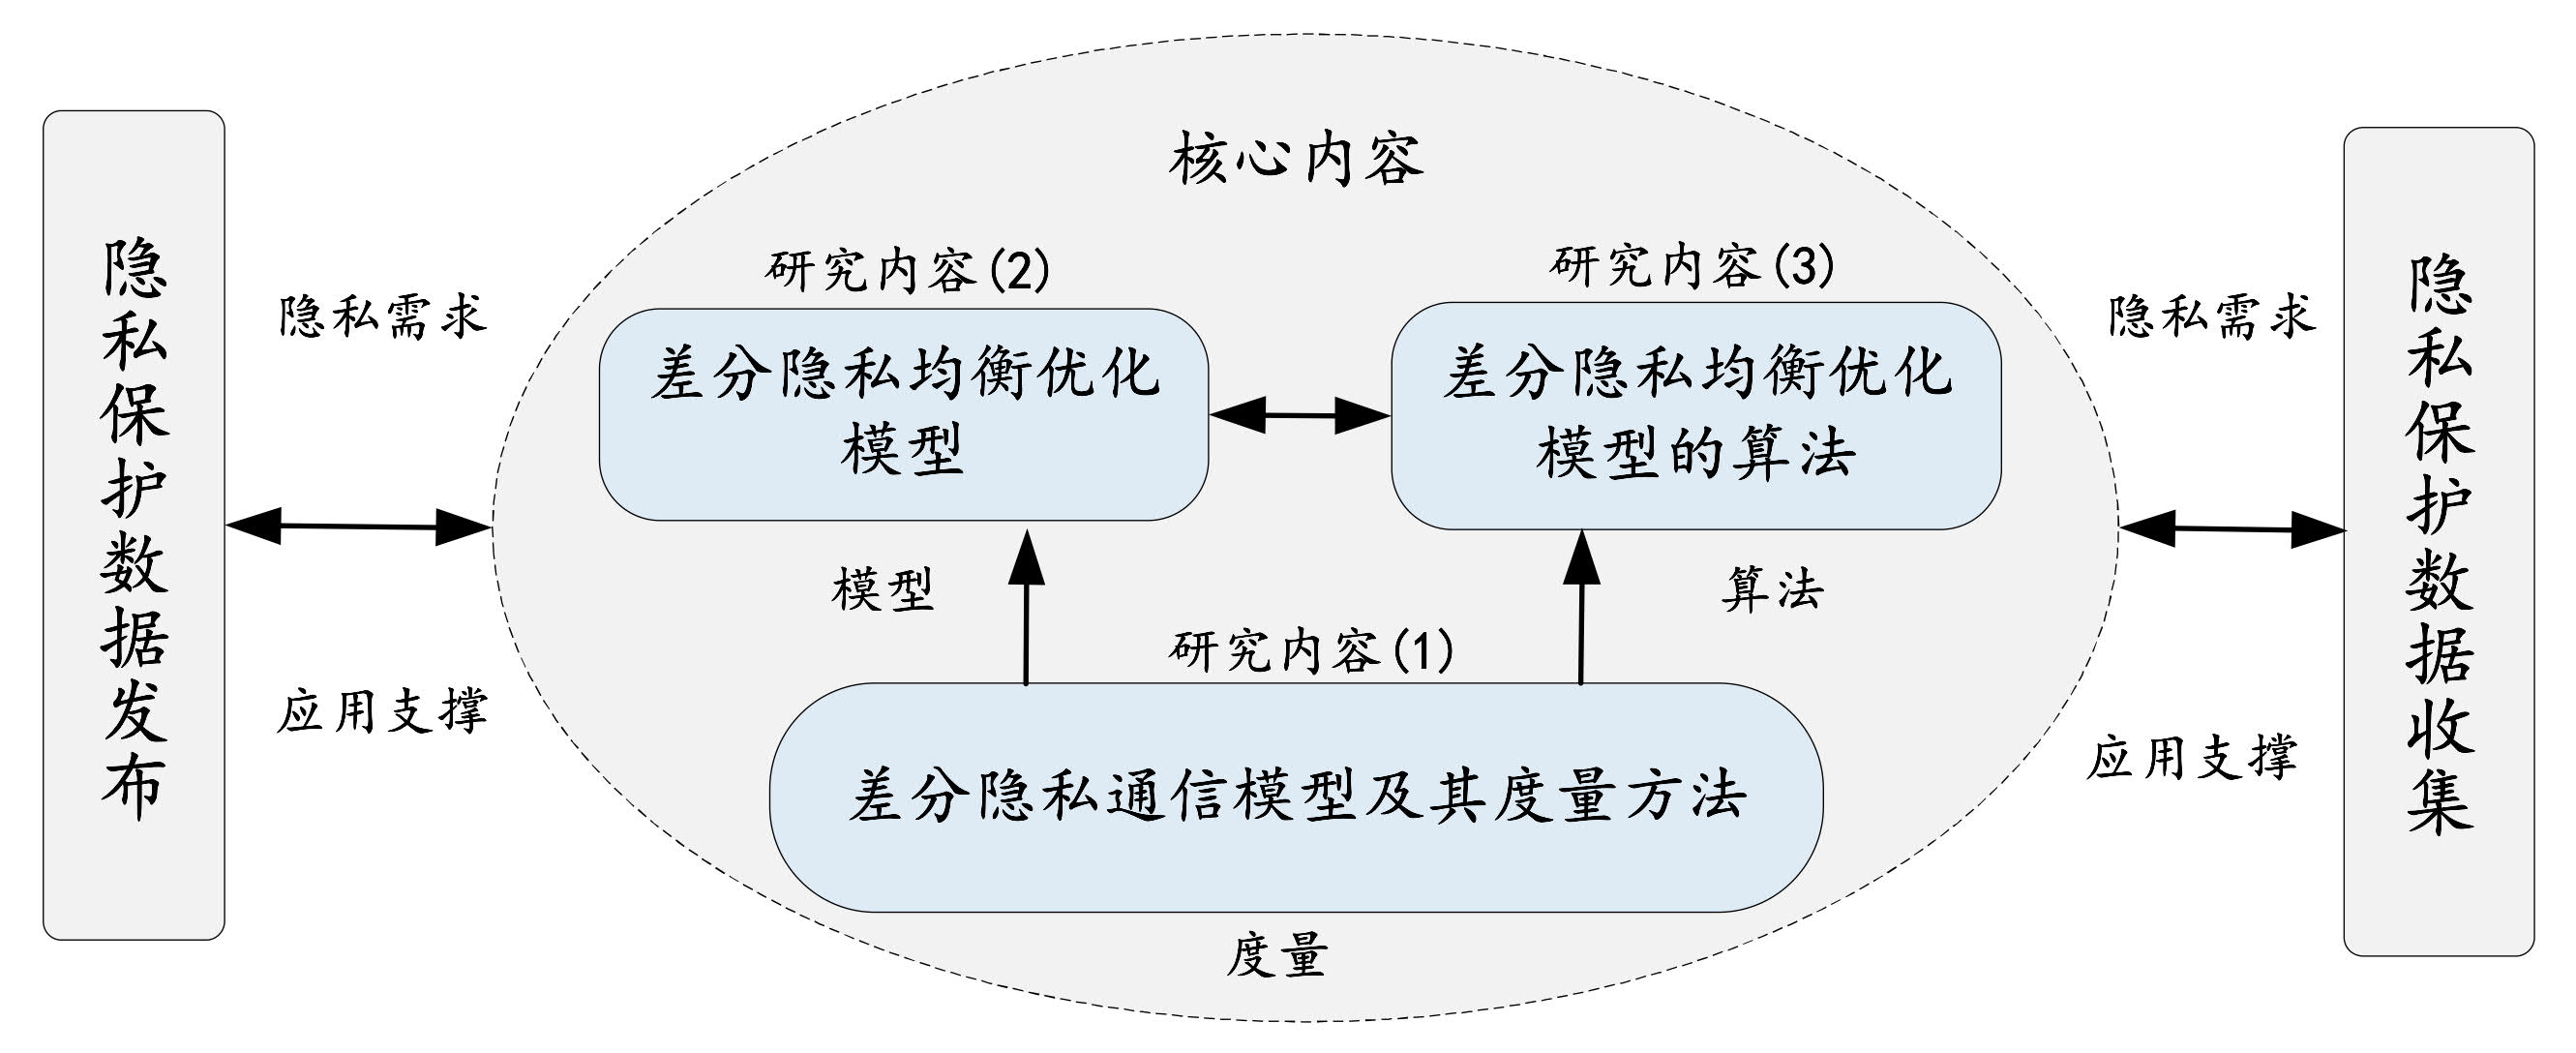
\includegraphics[width = 0.8\linewidth]{./figures/chapter01_1.jpg}
	\caption{本文核心研究内容及其关系}
	\label{fig:chapter1-research-relation}
\end{figure}

针对上述研究内容,本文在国家自然科学基金项目``理性隐私计算及隐私风险可控技术研究''的资助下,针对差分隐私保护模型开展了隐私信息熵度量、均衡与优化模型、隐私机制设计以及算法等方面的研究。本文的主要贡献是针对差分隐私多维及关联数据隐私保护的隐私与效用权衡问题,提出差分隐私的信息熵度量模型,权衡隐私与效用的均衡、优化模型及隐私机制设计方法。具体取得的主要成果有:
%\begin{enumerate}[\hskip 2em (1)]
%\item {\em 差分隐私通信模型及隐私度量}
%
%以差分隐私的概率性响应为基础,借鉴Shannon基本通信模型构建差分隐私的基本通信模型及其形式化表述。以此为基础,考虑差分隐私不同应用场景中的隐私攻击者(敌手)模型
%\item {\em 差分隐私均衡优化模型}
%
%\item {\em 差分隐私均衡优化模型的算法研究}
%\end{enumerate}

(1) {\em 差分隐私通信模型及其度量方法}
%分两段写,第一段写问题,第二段写本文的成果陈述

差分隐私的随机响应机理与信息论的噪声信道机制工作原理不谋而合,具有自然的相似性。以此为基本出发点,信息论方法被应用到差分隐私的研究中,并获得了一定的研究基础。在此方面,信息熵、条件熵、互信息量、率失真等基础方法均获得了具体的应用。但是,综述发现存在的工作中大多针对单一的敏感属性,拓展到多维属性的研究还相对较少。此外,现实中的多维属性极少存在相互独立的情景,大多存在数据关联,这种关联的相关性会增加个体隐私被推断的风险。然而,目前的研究尚缺失多维属性关联的差分隐私度量工作。


针对上述提到的问题,本文首先基于差分隐私的随机化响应原理,借鉴Shannon基本通信模型构建差分隐私的基本通信模型,并给出其形式化表述。以此基本通信模型为基础,考虑差分隐私不同应用场景中的隐私攻击者(敌手)模型,提出差分隐私通信模型中含背景知识的通信模型。在隐私度量方面,以基本的信息熵、条件熵、互信息量为基础,分别针对独立与关联的情景,提出了面向多维属性的隐私度量模型,给出了定量的信源熵、互信息量、联合熵、条件互信息的度量函数。进一步,在面向多维属性关联的差分隐私数据发布中,基于图模型、马尔可夫模型等,提出了多维属性关联的差分隐私信息泄露度量模型及方法。在数据效用度量方面,本文以构建的差分隐私通信模型为基础,借鉴信息论中的率失真理论,利用失真函数(损失函数)从数据重构的视角量化扰动数据表达原始数据的失真程度,给出了多维属性的效用度量,即是数据质量。最后,在度量随机扰动对多维数据关联的影响时,基于相关度度量、图理论,提出了多维数据关联依赖图的结构信息(Structural Information)度量方法。



(2) {\em 差分隐私均衡优化模型}

在差分隐私的应用中,隐私泄露风险及数据可用性与所使用的隐私保护机制密切相关。为了获得理想的隐私保护效果和合理的数据质量,差分隐私的最优化机制问题一直都是学术研究的焦点。学术研究进行了有意义的探索,存在的工作中已提出了一些最优的差分隐私方案。首先是针对``是'' 和`` 否''的问题,提出了二元数据的最优随机响应方案。其次,将问题扩展到类别型数据的多元随机响应方案。注意到,诸如此类的差分隐私方案将属性域的笛卡尔积作为信源字母表。如此以来,直接扩展上述方案到多维属性时,由于数据稀疏、域值空间大的问题,给隐私机制带来新的挑战。例如,在处理效率和数据效用方面性能打折。此外,在一些应用中可能是消息灵通的敌手模型,即有关数据拥有一定的先验知识。更有甚者,隐私攻击可以是策略型的敌手模型,这样的敌手不是像传统模型中考虑的敌手在观察到扰动数据后被动的攻击,相反,策略型的敌手可以与隐私保护系统进行交互,利益驱使他们偏爱最大收益的策略\cite{alvim2017information,alvim2018leakage}。针对这些问题的研究还不充分,促使研究者提出新的差分隐私机制方案。


%鉴于此,差分隐私机制设计的研究尚需要进一步深入推进。

针对上述问题,本文以差分隐私基本通信模型及其度量为基础,利用信息论、优化理论以及博弈均衡理论,提出了权衡隐私与数据效用的差分隐私均衡优化模型。首先,分析隐私保护系统参与者的隐私目标,利用信息熵度量模型及方法,将数据发布系统中数据发布的目标表达为给定数据失真约束条件下互信息隐私泄露的最小化问题,给出基本的优化模型。随后,在基本通信模型基础上引入含背景知识的敌手推断模型,提出了背景知识关联的差分隐私最优化模型,用于数据发布的差分隐私机制设计。此外,在隐私保护的多维数据收集场景中,形式化表达了互信息隐私与失真的优化模型,并进一步将其推广到多维数据情景,设计了面向多维数据收集的有序随机响应扰动(Orderly Randomized Response Perturbation,ORRP) 方案。更多地,在基础通信模型中考虑了策略型的敌手模型,基于量化信息流(QIF) 提出了隐私保护的攻防博弈(Privacy-Preserving Attack and Defense,PPAD)模型,并从博弈均衡的角度分析了差分隐私的最优策略行动。基于冯$\cdot$ 诺依曼- 摩根斯坦效用理论,理性的策略选择为等价的差分隐私机制提供了一种机制比较的方法。最后,分析表明均衡策略是最差情况的隐私泄露上界,其可用于评估隐私风险。


(3)  {\em 差分隐私均衡优化模型的算法}

本文研究的差分隐私最优化机制,在设计过程中主要包含有两个阶段:第一,依据系统的隐私、效用目标形式化一个均衡优化模型,并求解提出的模型计算出最优化隐私机制的概率分布函数;第二,根据得到的概率分布函数设计出具体的隐私保护方案实现隐私数据的随机扰动。鉴于此,对于所提出的差分隐私均衡优化模型求解的问题,算法的研究是个关键。本文研究在算法方面获得的主要成果有:


首先,针对差分隐私数据发布应用中敌手背景知识关联情景,本文修改了率失真函数,提出最优互信息隐私与失真模型,形式化模型表述与著名的率失真(Rate-distortion)函数具有相似的形式。由此,借鉴率失真求解的双重交替最小化Blahut-Arimoto~(B-A)算法\cite{blahut1972computation,arimoto1972an}提出了隐私与失真模型的求解算法,并给出了算法的计算复杂性分析。其次,针对差分隐私的本地化应用,使用B-A算法作为基本的构建模块,设计了有序随机响应扰动(ORRP)方案的实现算法,遵循两个阶段实现随机元组扰动。此外,针对多维数据关联损失度量问题,设计了多维属性相关度分析及关联损失量化的算法,并从理论上分析了所设计算法的计算复杂性。最后,对于本文所提出的隐私保护攻防博弈(PPAD)模型,基于交替最优响应策略选择,设计了均衡计算的策略优化选择算法。对于算法的研究增强了理论模型的可行性,与所提出的理论模型相辅相成。



\section{论文组织结构}
本文研究了差分隐私数据发布、数据收集场景中隐私与数据效用权衡的差分隐私均衡优化模型与算法。全文共分为七章,组织结构如图\ref{fig:chapter1-research-structure}所示,各章节内容的具体安排如下:

\begin{figure}[htbp]
	\centering
	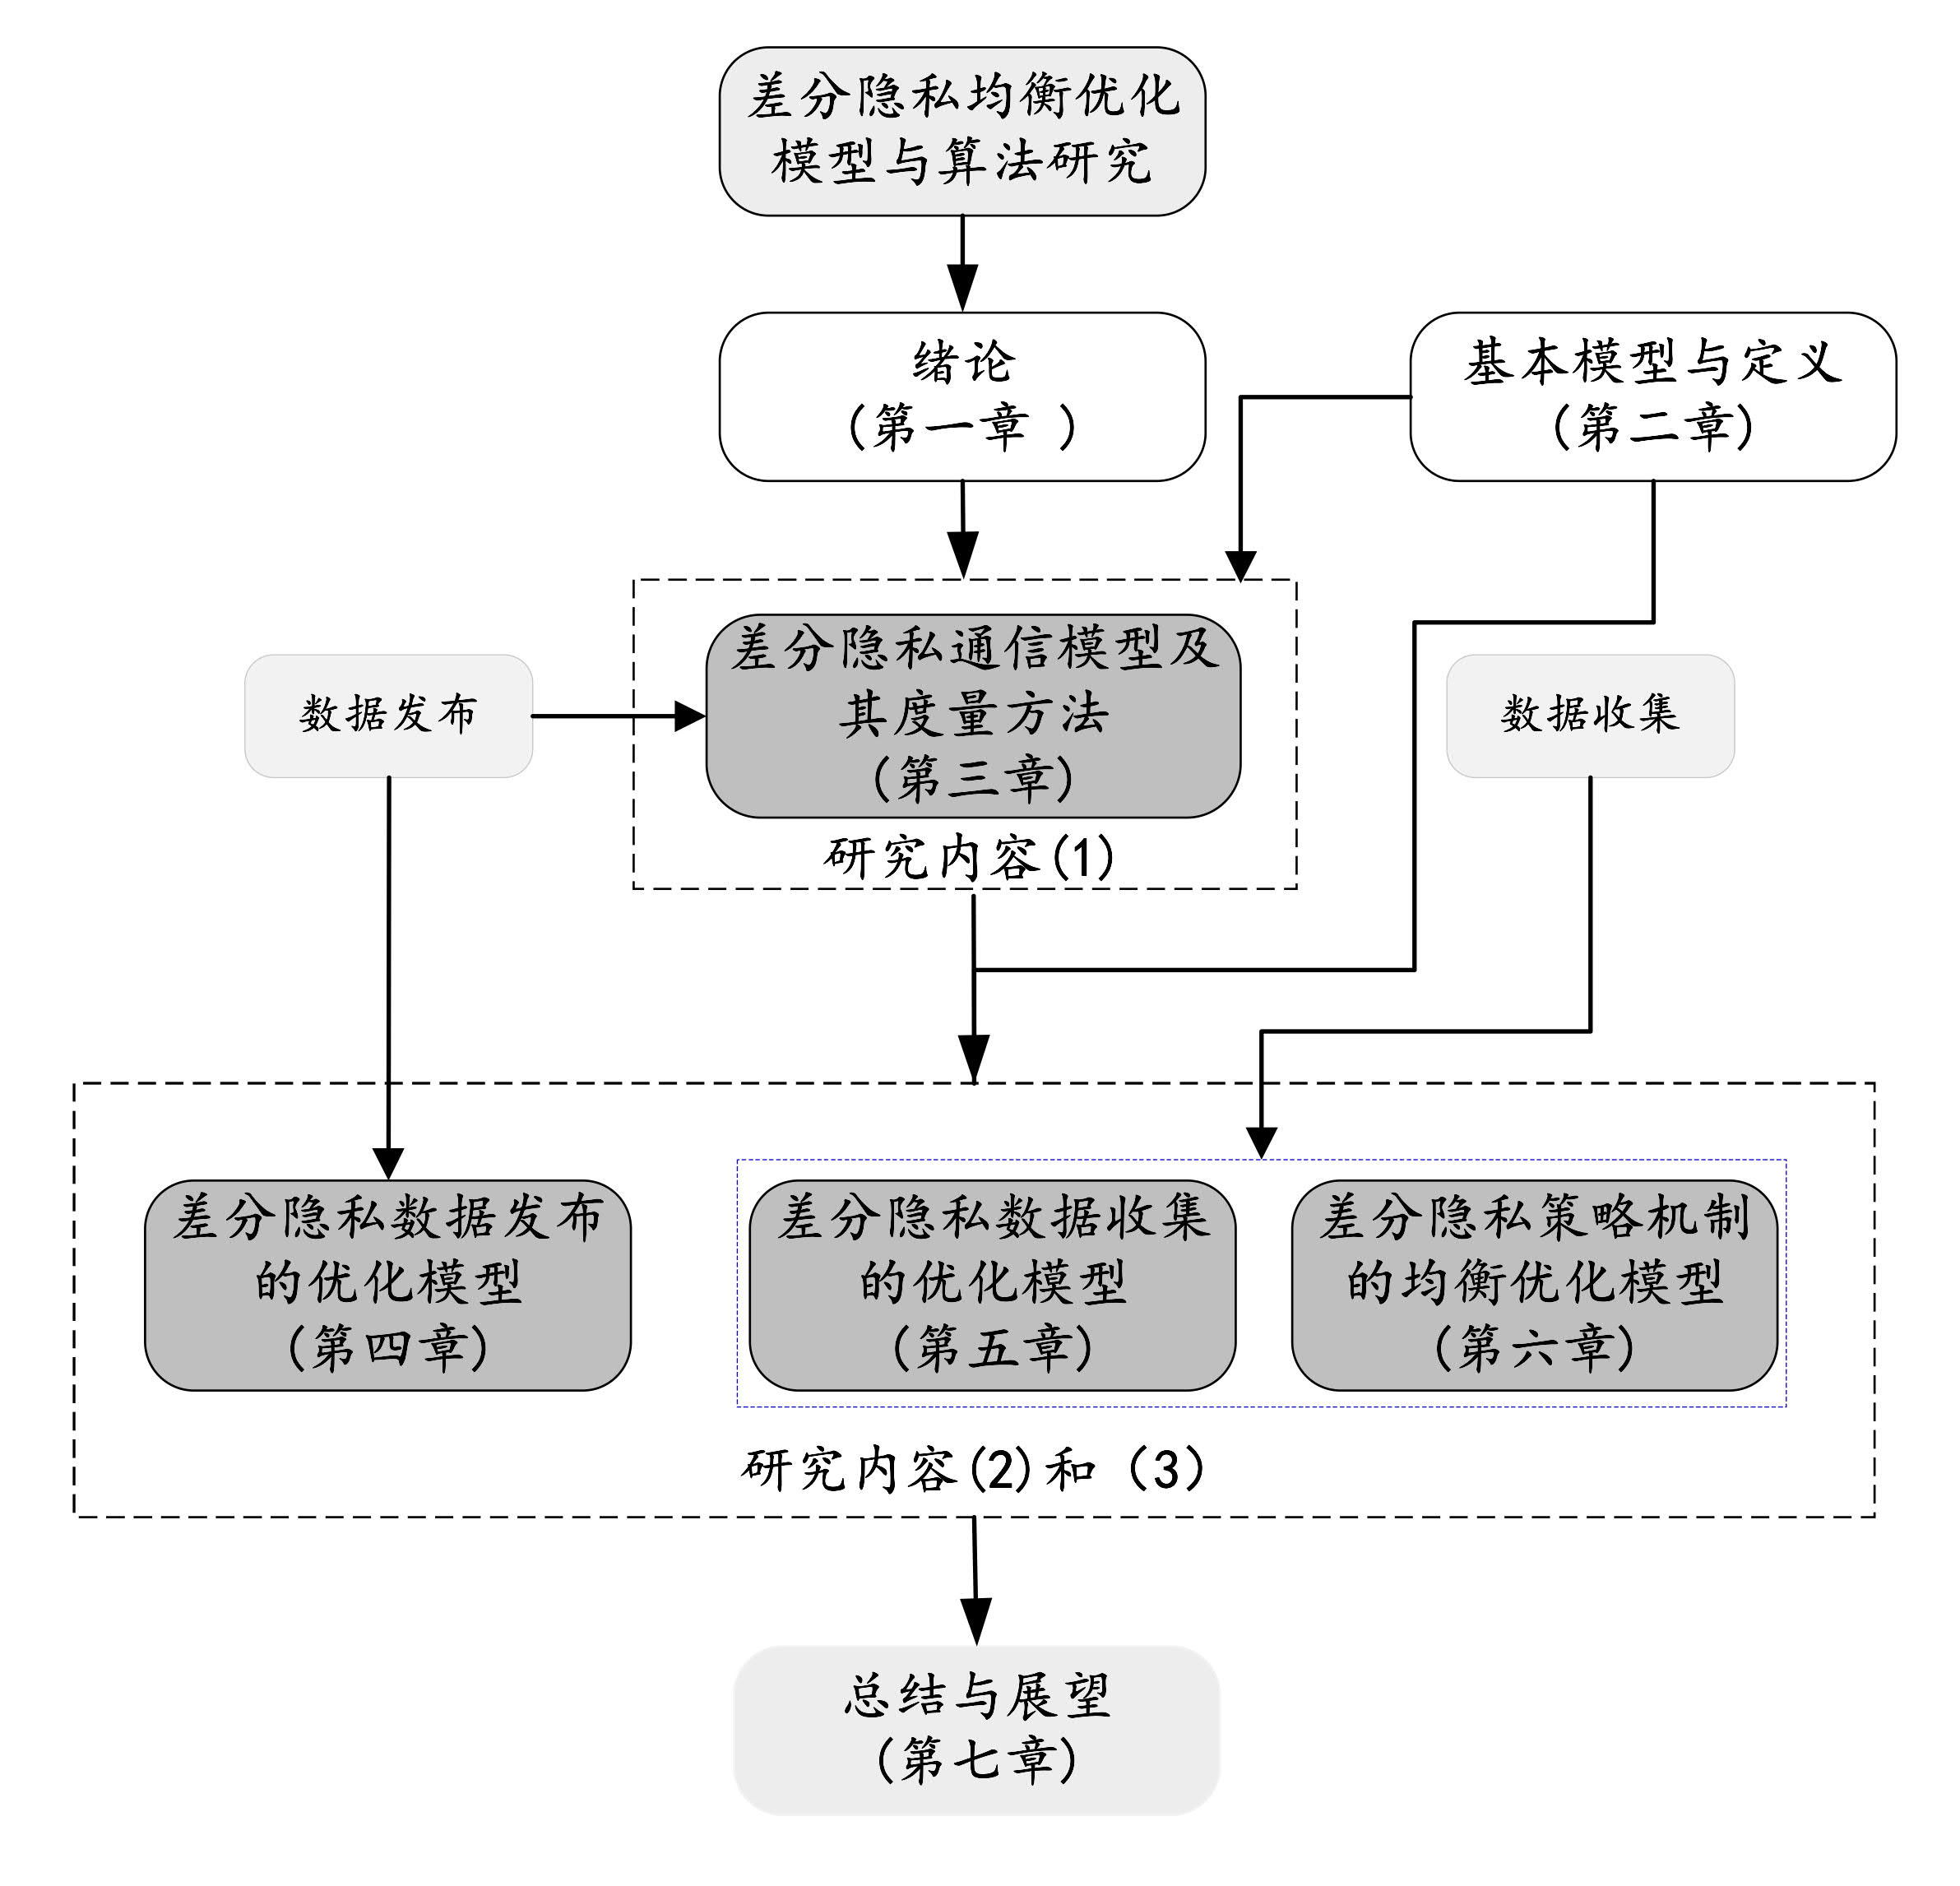
\includegraphics[width = 0.7\linewidth]{./figures/chapter01_2.jpg}
	\caption{本文的章节内容组织结构图}
	\label{fig:chapter1-research-structure}
\end{figure}

第\ref{chapter01}章为\textit{绪论},首先阐述了本文的研究背景及意义,随后针对差分隐私分析了存在的问题,凝练出本文研究需要解决的关键问题。基于上述分析,阐述了本文的研究内容和研究取得的主要成果。最后给出了本文的章节组织结构安排。



第\ref{chapter02}章为{\em 基本模型与定义},介绍了本文研究所使用的基本模型与定义。首先,给出了隐私、隐私泄露的定义,并阐述了差分隐私模型及定义。其次,叙述了Shannon信息论的通信模型,引入信息熵、条件熵、联合熵、互信息量等概念,以此为基础介绍了数据处理不等式、费诺不等式和率失真理论等内容。随后,阐述了最优化问题、对策博弈以及凹凸博弈的相关知识。最后,以上述为基础,给出了本文中差分隐私均衡优化的定义,界定后续研究的范畴。


第\ref{chapter03}章为{\em 差分隐私通信模型及其度量方法},建立差分隐私与信息论的基本联系,奠定本文的研究基础。首先,基于Shannon基本通信模型,介绍了差分隐私基本通信模型,并给出了形式化的模型表达。其次,以差分隐私的基本通信模型为基础,引入信息熵、互信息、失真的概念对隐私与效用进行度量,提出信息熵度量模型及方法。进一步,在基本的度量基础上,针对多维关联属性的情景,提出面向关联属性的差分隐私信息熵度量方法,本章中的度量模型及方法为开展后续章节的研究奠定了基础。

第\ref{chapter04}章为{\em 差分隐私数据发布的优化模型},研究了隐私与数据效用权衡的最优差分隐私机制。首先,基于第\ref{chapter02}章基础、第\ref{chapter03}章差分隐私通信模型及度量方法,分析了隐私系统的目标,借鉴率失真理论构建了面向差分隐私数据发布的优化模型。其次,在基本的通信模型基础上引入敌手模型,并考虑了敌手拥有关联辅助背景知识对隐私泄露的影响,提出了基于联合事件的互信息隐私度量。随后,修改率失真表述形式,提出了最小化隐私泄露的优化模型,用于获得隐私机制的概率分布函数。此外,设计了互信息隐私最优信道机制的近似迭代求解算法,并给出具体的验证分析。

第\ref{chapter05}章为{\em 差分隐私数据收集的优化模型},围绕隐私保护机制设计的两个阶段,研究了面向数据收集的多维数据最优隐私机制。首先,以第\ref{chapter03}章的度量为基础,形式化互信息隐私(MI-privacy)最优化模型,设计模型求解算法寻找最优机制的概率密度函数。随后,将其作为基本构建模块应用到多维数据,提出有序随机响应扰动(ORRP)方案。最后,针对提出的ORRP方案,介绍了隐私、数据效用以及相关度损失的评估与分析,并利用真实数据集给出了所提方案的实验分析。


第\ref{chapter06}章为{\em 差分隐私策略机制的均衡优化模型},应用博弈均衡理论研究了差分隐私策略机制选择问题。通过分析隐私保护系统参与者的隐私目标,基于信息熵度量模型及方法将隐私目标形式化为隐私泄露的极大极小问题。然后,分析系统参与者的可行策略,构建了隐私保护的攻防博弈(PPAD)模型。针对本文关注的应用,实例化PPAD为两方零和对策博弈模型,并提供了均衡的理论分析以及算法实现。最后,阐述了均衡在隐私保护中的内涵及意义。


第\ref{chapter07}章为\textit{总结与展望},首先总结了本文的研究工作,进一步,展望了未来研究工作的方向和重点。


